\section{Results}
\label{sec:results}

\para{Aggregate comparison.} \Tabref{tab:aggregate-results} shows the main aggregate outcome. L2 increases mean test accuracy from $0.8267$ to $0.8385$, but the mean paired gain is only $+0.0118$ with a $95\%$ confidence interval of $[-0.0075, 0.0311]$ and $p=0.205$. Weighted F1 shows the same pattern: a small mean gain of $+0.0100$ with $p=0.302$. In contrast, the train-validation gap drops from $0.1297$ to $0.0257$, a mean paired change of $-0.1040$ with $p=0.011$ and paired Cohen's $d=-0.878$. This is the clearest statistically supported effect in the study.

\begin{table*}[t]
    \centering
    \resizebox{\textwidth}{!}{%
    \begin{tabular}{@{}lccccccl@{}}
        \toprule
        Metric & Baseline Mean & L2 Mean & Mean Diff. ($\Delta$) & 95\% CI for $\Delta$ & $p$-value & Paired $d$ & Better \\
        \midrule
        Test accuracy & 0.8292 & {\bf 0.8385} & +0.0093 \increase & [$-0.0114$, $0.0300$] & 0.345 & 0.285 & L2 \\
        Weighted F1 & 0.8276 & {\bf 0.8357} & +0.0081 \increase & [$-0.0138$, $0.0301$] & 0.431 & 0.236 & L2 \\
        Train-val gap & 0.1297 & {\bf 0.0257} & -0.1040 \decrease & [$-0.1792$, $-0.0287$] & {\bf 0.011} & -0.878 & L2 \\
        \bottomrule
    \end{tabular}%
    }
    \caption{Aggregate paired comparison across 12 dataset-seed pairs. Higher is better for accuracy and weighted F1, while lower is better for the train-validation gap. Best values are shown in \textbf{bold}. Only the gap reduction is statistically significant at $\alpha=0.05$.}
    \label{tab:aggregate-results}
\end{table*}


\para{Per-dataset behavior.} \Tabref{tab:dataset-results} shows that the aggregate average hides substantial dataset heterogeneity. \breastcancer and \wine both favor L2 on accuracy and weighted F1, with \wine reaching perfect mean test accuracy under the selected settings. \sonar and \glass show the opposite pattern: L2 shrinks the train-validation gap strongly but does not improve mean test accuracy. This split is important because it shows that reduced overfitting pressure does not automatically imply better test performance.

\begin{table*}[t]
    \centering
    \resizebox{\textwidth}{!}{%
    \begin{tabular}{@{}lccccccc@{}}
        \toprule
        Dataset & Dummy Acc. & Baseline Acc. & L2 Acc. & Baseline F1 & L2 F1 & Baseline Gap & L2 Gap \\
        \midrule
        \breastcancer & 0.558 & 0.946 & {\bf 0.977} & 0.946 & {\bf 0.977} & 0.027 & {\bf -0.011} \\
        \wine & 0.321 & 0.963 & {\bf 1.000} & 0.963 & {\bf 1.000} & 0.049 & {\bf 0.019} \\
        \sonar & 0.448 & {\bf 0.802} & 0.781 & {\bf 0.802} & 0.780 & 0.301 & {\bf 0.049} \\
        \glass & 0.273 & {\bf 0.596} & {\bf 0.596} & {\bf 0.592} & 0.586 & 0.141 & {\bf 0.046} \\
        \bottomrule
    \end{tabular}%
    }
    \caption{Per-dataset mean results across three seeds. Higher is better for accuracy and weighted F1, and lower is better for the train-validation gap. The pattern is mixed for predictive metrics but consistently favors L2 for gap reduction. Median selected $C$ values are $0.10$ for \breastcancer, $0.01$ for \wine, $0.10$ for \sonar, and $100.0$ for \glass.}
    \label{tab:dataset-results}
\end{table*}


\para{How consistent is the overfitting reduction?} The run-level counts sharpen the interpretation. L2 improves test accuracy in $5/12$ runs, matches the baseline in $5/12$, and worsens it in $2/12$. By contrast, it reduces the train-validation gap in $11/12$ runs. The regularization effect is therefore far more stable for shrinkage and gap control than for final predictive accuracy.

\para{Regularization sweep and shrinkage.} \Figref{fig:reg-summary} summarizes the validation sweep. The wine example shows that intermediate values of $C$ can reach perfect validation and test performance while keeping coefficients much smaller than the near-unregularized baseline. Across datasets, the selected median $C$ values vary from $0.01$ on \wine to $100$ on \glass, which reinforces that the best amount of regularization is data dependent rather than universal.

\begin{figure*}[t]
    \centering
    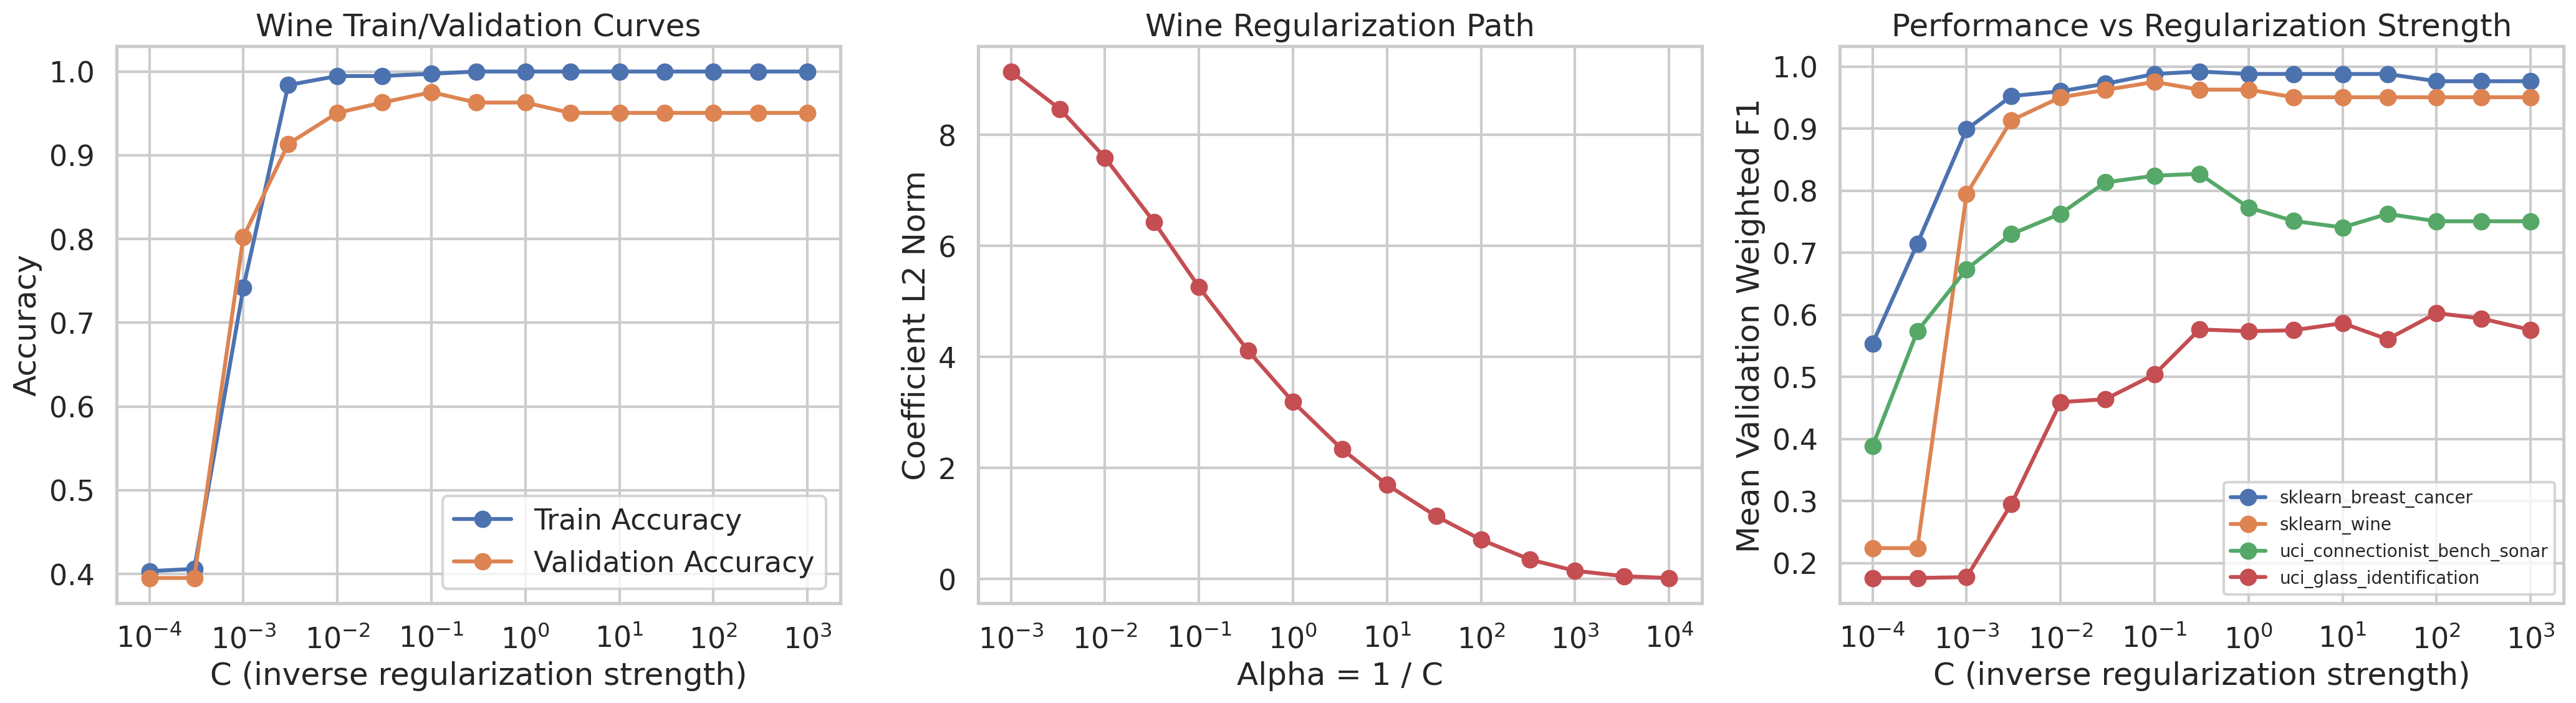
\includegraphics[width=0.95\linewidth]{figures/regularization_summary.png}
    \caption{Regularization summary figure from the experiment artifacts. \figleft shows train and validation curves on \wine across the L2 sweep. \figcenter shows coefficient shrinkage along the same path. \figright aggregates validation weighted F1 as a function of $C$ across datasets. The figure highlights the central pattern of the paper: performance can improve at intermediate regularization strengths, but the location and size of the gain vary by dataset.}
    \label{fig:reg-summary}
\end{figure*}

\para{Distribution of train-validation gaps.} \Figref{fig:gap-boxplot} shows the gap distribution by dataset. The largest contraction appears on \sonar, where the mean gap drops from $0.3011$ to $0.0486$. \glass also shows a large reduction, from $0.1408$ to $0.0455$. The visual pattern matches the paired test: L2 acts as a strong anti-overfitting mechanism even when accuracy gains are weak or absent.

\begin{figure}[t]
    \centering
    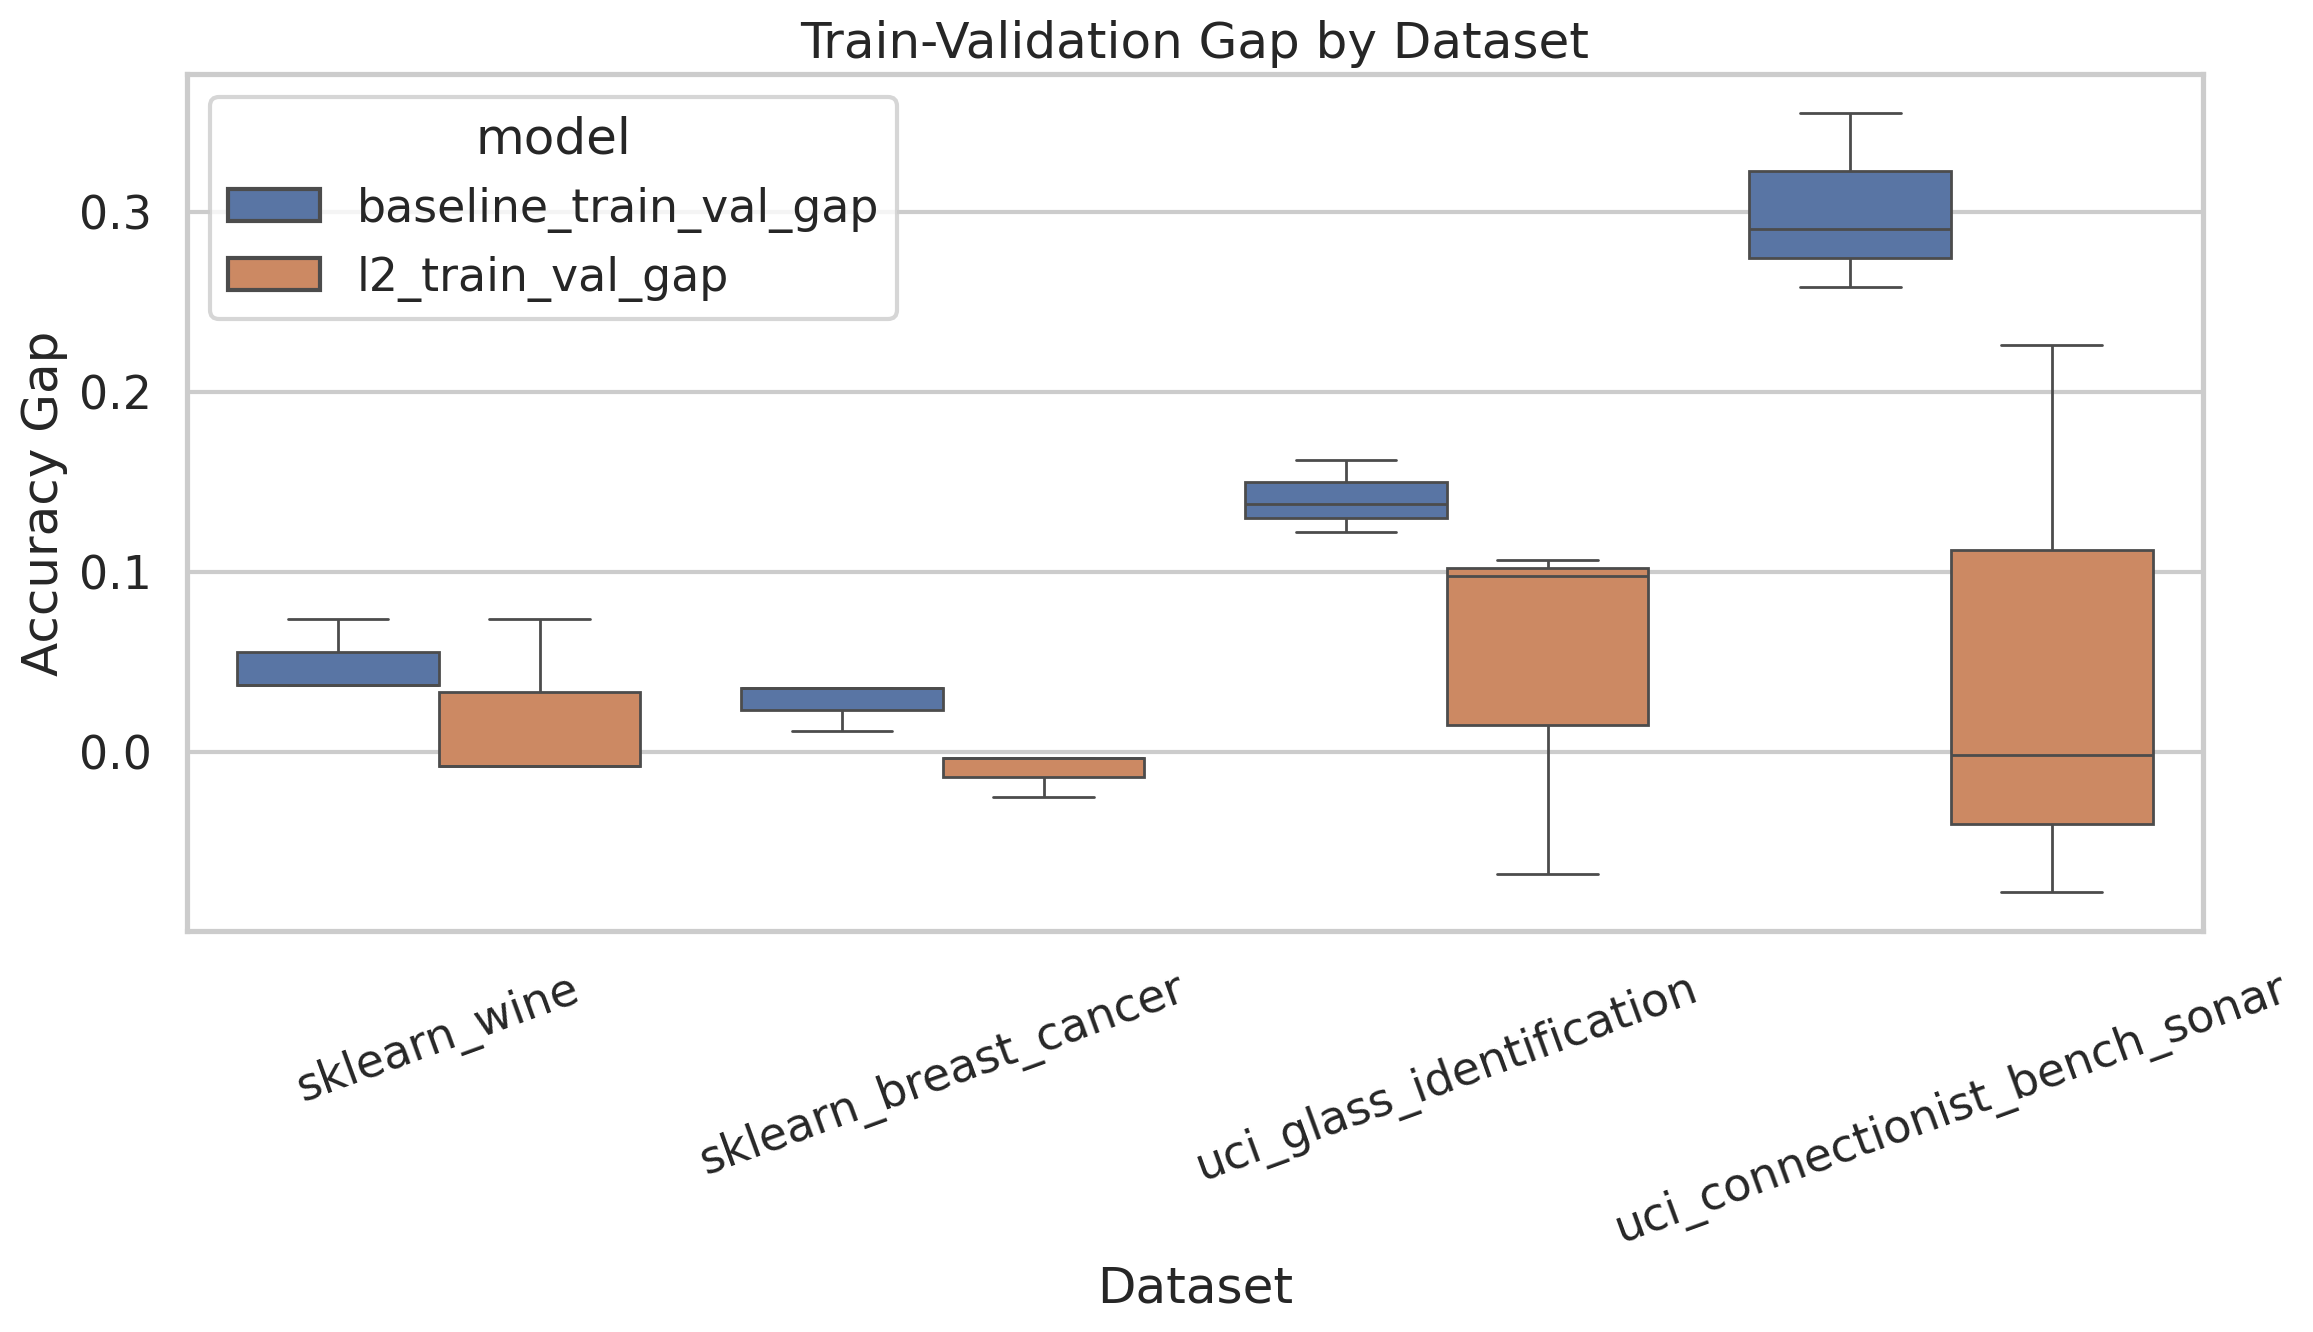
\includegraphics[width=0.95\linewidth]{figures/train_val_gap_boxplot.png}
    \caption{Train-validation accuracy gap by dataset for the near-unregularized baseline and the validation-tuned L2 model. Lower is better. L2 reduces the gap for nearly every run and produces the clearest effect on the harder small datasets, especially \sonar and \glass.}
    \label{fig:gap-boxplot}
\end{figure}

\para{Sensitivity analysis.} The L2 sweep also serves as a simple ablation on regularization strength. Extremely small $C$ values underfit, as expected, while very large $C$ values recover the high-norm near-unregularized regime. The useful region lies in between, but that region differs by dataset. This is consistent with our main conclusion: regularization helps most as a controllable bias-variance tradeoff, not as a uniform test-accuracy improvement.
